% RWC 2027 contributed talk proposal: zkEMV.
% CFP https://rwc.iacr.org/2027/contributed.php.

\documentclass[10pt,a4paper]{article}

\usepackage[T1]{fontenc}
\usepackage{newtxtext,newtxmath}
\usepackage[margin=2cm]{geometry}
\usepackage{microtype}
\usepackage{booktabs}
\usepackage{enumitem}
\usepackage{tikz}
\usetikzlibrary{arrows.meta,positioning}
\usepackage[hidelinks]{hyperref}

\setlist{nosep}

\title{zkEMV: Private Credentials from EMV Offline Data Authentication}
\author{Anjan Roy (presenting author)\\Radboud University and Avail\\\texttt{anjan.roy@ru.nl}}
\date{October, 2026}

\begin{document}
\maketitle

\begin{abstract}
  % problem
  Online services offering a free tier, such as AI inference tokens or GPU compute credits, face abuse from users creating many accounts: Stripe reports that 7.4\% of sign-ups at AI company websites are suspected multi-account abuse.
  The usual defence is to verify a phone number, a government-issued identity card or a payment card, which makes the service hold personally identifiable information (PII), a lucrative target for hackers, and turns away privacy-conscious users.
  % insight
  EMVCo reports over 15.6 billion EMV chip cards are in use.
  Each chip-card authenticates itself to readers through an \emph{offline data authentication} (ODA) step, signing a fresh challenge with a key that an RSA certificate chain ties to the certification authority (CA).
  But these certificates embed the card number, so verifying the chain server-side means handing over the card number itself.
  % zkEMV
  In \emph{zkEMV}, the user taps their contactless card on their own NFC-capable device, which proves locally in zero knowledge that a genuine EMV card signed the verifier's challenge and that its certificates have not expired.
  It needs no change to card chips, issuers or payment networks, and unlike zero-knowledge credentials over mdoc or OpenID Connect, no enrolment with a government or a trusted identity provider.
  To the best of our knowledge, this is the first work on zero-knowledge proof of EMV ODA.
  % verifier pov
  The verifier checks the proof against the CA public key it trusts, without ever seeing the card number, expiry dates or certificates.
  It only learns a 32-byte nullifier which is deterministic for a card within a verifier-scope, and unlinkable across scopes, plus optionally requested card attributes, such as issuing country or whether it is a credit card.
  % perf
  Proving runs entirely on the user's own device: on a Samsung Galaxy S25 Ultra running on battery power, it takes 700ms for a Visa card and 850ms for a Mastercard, and verification takes under 100ms.
  % summarise
  The talk presents the zkEMV protocol and its security model, followed by a live demo.
  We hope it opens the door for discussion among stakeholders on how to design the future of human and agentic payment protocols in a more privacy-preserving way.
\end{abstract}

\section{Motivation}

% problem
Any online business offering a free tier, such as AI inference tokens, GPU compute credits, CI run minutes, a privacy-focused virtual private network (VPN) or an email relay, faces abuse from spammers, often degrading the quality of service (QoS) for real customers.
Stripe reports that 7.4\% of sign-ups at AI company websites are implicated in suspected multi-account abuse~\cite{stripe-abuse}, and after a massive uptick in crypto mining on free CI minutes, GitLab began requiring new free-tier customers to provide a valid payment card~\cite{gitlab-crypto-mining}.
Fly.io required a card even for its free services, not to charge it, but to keep out VMs mining cryptocurrencies~\cite{flyio-free-postgres}, and Heroku phased out its free plans altogether in 2022, citing the effort of managing their fraud and abuse~\cite{heroku-next-chapter}.
This abuse is the classic Sybil attack~\cite{DBLP:conf/iptps/Douceur02}: without a trusted authority certifying identities, one user can always pose as many.

% solution
Service providers resort to collecting identifying user data, to stop spammers from easily creating new identities.
The usual defences are verifying a phone number, uploading a government-issued identity card, or adding a payment card.
These let service providers deduplicate user accounts and limit resource usage to unique users.
For convenience, major card networks such as Visa and Mastercard offer tap-to-verify products~\cite{visa-tap,mc-tap-to-verify}.
% new problem
But this opens the door to a bigger problem: service providers must carefully handle any personally identifiable information (PII) they collect, because it is a lucrative target for hackers.
Privacy-conscious customers, aware of such data breaches, prefer not to put their card number, expiry date or CVV on a random website, which leaves them unable to try out a product or service.

Surprisingly, every chip card already holds the cryptographic foundation for a much more privacy-respecting authentication mechanism.
% no ZK
During ODA, a contactless card sends the reader a certificate chain and a signature over the reader's fresh challenge, made with the private key held inside the chip~\cite{emv-book2}.
These credentials are already issued and in circulation, with almost 15.6 billion EMV chip cards in use~\cite{emvco-stats}, unlike Privacy Pass~\cite{privacypass} and Private Access Tokens~\cite{apple-pat}, which rely on a platform attester.
% problem
However, the EMV certificates embed the card number, formally the primary account number (PAN), so verifying the certificate chain server-side means handing over identifying user data.
% with ZK
Zero-knowledge cryptography comes to the rescue: the user's device produces a zero-knowledge proof (ZKP) over the certificate chain without exposing the PAN.
% differentiation
Zero-knowledge proofs over existing credentials, such as mdoc with ECDSA~\cite{DBLP:journals/cic/FrigoS26}, JWT and mDL~\cite{DBLP:journals/iacr/PaquinPZ24}, OpenID Connect~\cite{DBLP:conf/ccs/BaldimtsiC0LMR024} and legacy signatures~\cite{DBLP:conf/sp/WooOSPG25}, need enrolment with a government or a trusted identity provider.
To the best of our knowledge, no earlier work proves EMV ODA in zero knowledge or explores the practical use cases it enables.

\section{The protocol}

There are two participants in the protocol: a user (prover) and a service provider (verifier).
The user has a near field communication (NFC) capable device and an EMV card in their physical possession.
The user proves to the service provider that they tapped a genuine EMV card on their device whose certificates have not expired as of verification time.

\paragraph{Flow.}
The verifier issues a challenge: a random 4-byte nonce, the current time at month-level granularity (\texttt{YY-MM}), a \emph{scope} and optional bits requesting card attributes derived from the bank identification number (BIN), i.e., the first 6 to 8 digits of the PAN.
The user's device fetches the challenge and checks that the requested scope matches the origin it authenticated over TLS.
The user taps the EMV card on their device, which forwards the nonce for signing by the card-held ICC private key.
The card returns the signature with both the issuer and ICC certificates, which chain up to the trust anchor~--- the CA public key.
The captured transcript of the NFC communication is fed into the ZK circuit for proving on the user's device.
The proof outputs a 32-byte nullifier, the Poseidon2~\cite{DBLP:conf/africacrypt/GrassiKS23} hash of the card's certified ICC public key and the scope.
On receiving the ZKP, the verifier checks that the proof's public inputs equal its challenge and that the CA key is one it trusts, then verifies the ZKP itself.

\begin{figure}[t]
\centering
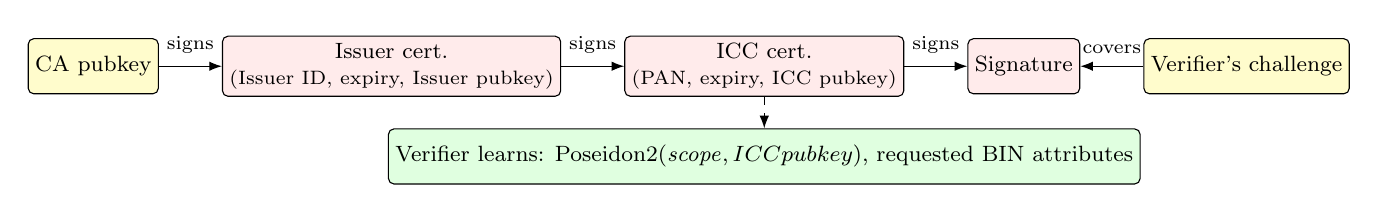
\begin{tikzpicture}[font=\footnotesize, node distance=8mm,
  box/.style={draw, rounded corners=2pt, inner sep=2.5pt, align=center, minimum height=7mm},
  arr/.style={-{Latex[length=1.6mm]}}]
  \node[box, fill=yellow!20] (ca) {CA pubkey};
  \node[box, fill=red!8, right=of ca] (iss) {Issuer cert.\\\scriptsize (Issuer ID, expiry, Issuer pubkey)};
  \node[box, fill=red!8, right=of iss] (icc) {ICC cert.\\\scriptsize (PAN, expiry, ICC pubkey)};
  \node[box, fill=red!8, right=of icc] (sdad) {Signature};
  \node[box, fill=yellow!20, right=of sdad] (nonce) {Verifier's challenge};
  \draw[arr] (ca) -- node[above=1pt]{\scriptsize signs} (iss);
  \draw[arr] (iss) -- node[above=1pt]{\scriptsize signs} (icc);
  \draw[arr] (icc) -- node[above=1pt]{\scriptsize signs} (sdad);
  \draw[arr] (nonce) -- node[above=1pt]{\scriptsize covers} (sdad);
  \node[box, fill=green!12, below=4mm of icc] (out) {Verifier learns: $\mathrm{Poseidon2}(\mathit{scope}, \text{ICC pubkey})$, requested BIN attributes};
  \draw[arr, dashed] (icc.south) -- (out.north);
\end{tikzpicture}
\caption{The ODA certificate chain proved in zero knowledge.}
\label{fig:chain}
\end{figure}

\paragraph{Statement.}
The public inputs to the circuit are the CA public key, nonce, time, scope, and the optional attribute bits with a BIN-table Merkle root.
% cert chain
As depicted in Figure~\ref{fig:chain}, three RSA signatures are verified along the EMV certificate chain, each recovering the signed message as $\texttt{msg} = \texttt{sig} ^ 3 \bmod n$, where $n$ is the RSA modulus.
Each recovered message is parsed following ISO/IEC 9796-2~\cite{iso9796-2} message recovery, asserting its fixed header, trailer and format bytes.
The circuit then recomputes the SHA-1 hash~\cite{fips180-4} over the recovered message and checks it against the hash embedded in it.
Each recovered certificate holds the next public key in the chain, which continues the authenticity check.
Additionally, it enforces that the issuer identifier matches the PAN prefix and that neither certificate has expired as of the verifier-chosen \texttt{YY-MM}.
% nullifier
To prevent a malicious user from proving a forged statement, the circuit computes predicates only from bytes covered by the signatures in the certificate chain.
The nullifier is therefore deterministic for a card within a verifier-scope, and unlinkable across them.
% attributes
Optionally, the circuit reveals requested attributes without exposing the BIN, such as the issuing country, whether it is a credit, debit or prepaid card, its brand, and whether it is for commercial use.
It proves inclusion in a binary Merkle tree, built with Poseidon2 over ranges of the PAN's first 12 digits, against a Merkle root which the verifier commits to.

\section{Use cases}

zkEMV-based authentication helps wherever fake accounts drain resources from real users and no actual payment needs to happen.
Users do not need to trust a random website with their card details, and the website's database no longer holds card data for hackers to steal.

\begin{itemize}
\item \textbf{Free tiers and trials}
A daily quota of LLM tokens for each account that proves possession of a genuine EMV card, without any risk of leaking customer data.
\item \textbf{Sticky banlists}
Discord communities which seek only well-mannered humans can maintain a banlist of scoped nullifiers, without ever seeing a user's card details or email address.
\item \textbf{One vote per card}
Polls and petitions allow only one participation per EMV card, while nullifiers stay unlinkable across events, preserving user privacy from a curious platform operator.
\item \textbf{Two-factor authentication}
Before any irreversible account operation, the user taps their EMV card on their phone to prove that it derives the enrolled nullifier.
\item \textbf{Bot friction}
Accepting a zkEMV proof is a privacy-respecting way to keep bots from spamming a service.
\end{itemize}

Additionally, services might impose constraints such as ``it needs to be a credit card issued in a specific country'' without learning the card number.
Anti-abuse aggregators such as Human Passport~\cite{human-passport} could accept a zkEMV proof as another signal.

\section{Client-side proving}

A zkEMV proof is generated on the user's own device, without the card data ever leaving it.
The Noir~\cite{noir} circuits are proved using ProveKit~\cite{provekit}, developed by World~\cite{world-provekit}.
ProveKit generates zero-knowledge proofs using a Spartan-based~\cite{DBLP:conf/crypto/Setty20} sumcheck protocol with the WHIR~\cite{DBLP:conf/eurocrypt/ArnonCFY25} hash-based polynomial commitment scheme, without any trusted setup.
Each EMV card profile gets its own circuit, since RSA key lengths differ between profiles.

\begin{table}[ht]
\centering
\begin{tabular}{@{}lcc@{}}
\toprule
& Visa fDDA & Mastercard DDA \\
\midrule
R1CS constraints & 64,702 & 93,054 \\
Prove on the phone & 660\,ms & 823\,ms \\
Verify & 85\,ms & 91\,ms \\
Proof size & 616.6\,KiB & 636.2\,KiB \\
\bottomrule
\end{tabular}
\caption{On a Samsung Galaxy S25 Ultra (Snapdragon 8 Elite, Android 16, 12\,GB RAM), on battery.}
\end{table}

\section{Limitations}

A zkEMV proof shows that a genuinely issued card was live and tapped, but that does not prove ``personhood'', since one person can easily hold multiple EMV cards.
If the client skips authenticating the verifier's origin, a malicious verifier can obtain the nullifier for another verifier's scope, which lets it track a user's presence across venues if a nullifier database leaks.
Because ProveKit proofs are zero-knowledge~\cite{world-provekit}, card data stays private against verifiers, but not against the card issuer or payment network.
Any merchant which has already seen a tap of an EMV card, i.e., captured its ICC public key, can compute its nullifier for any scope it can guess.
zkEMV inherits the security of EMV's ODA: SHA-1 has a practical chosen-prefix collision attack~\cite{DBLP:conf/uss/LeurentP20}, and ISO/IEC 9796-2 has well-studied forgery attacks~\cite{DBLP:conf/crypto/CoronNTW09}.
The RSA-896 challenge number was recently factored, setting a new record~\cite{weis-rsa896}, though EMVCo expects 1984-bit RSA keys to last until at least 2036~\cite{emvco-kl30}.
EMVCo specifies the elliptic curve Schnorr digital signature algorithm (EC-SDSA) over the NIST P-256 curve with SHA-256~\cite{emv-c8,emv-book-e}, but most issued contactless cards still rely on RSA for offline authentication~\cite{emvco-quantum}.
Even though a zkEMV verifier never sees the card's raw signatures over a 4-byte nonce, an attacker who harvests $k$ signatures from a card can impersonate it with probability $k \cdot 2^{-32}$ per challenge.

\section{Why RWC}

This talk introduces a new privacy-preserving credential to the RWC audience, built on infrastructure already in billions of people's hands, using modern zero-knowledge cryptography, and entirely provable on the user's device.
Its goal is to first show the audience how zkEMV wraps EMV's decades-old ODA protocol in a zero-knowledge proof, and then start an open discussion on the future design of EMV and agentic payments, so that the right guardrails get built into the protocol, protecting both user and agent privacy.
To give the audience a taste of practicality, the talk includes a live onstage demo.

\section*{Speaker}

\textbf{Anjan Roy} is a PhD candidate in applied cryptography at Radboud University, the Netherlands, supervised by Prof. Joan Daemen and Dr. Gilles Van Assche.
He also leads engineering of a zkAppchain at Avail, which powers privacy-preserving payments and DeFi on public blockchains.
He was previously a senior cryptography engineer at the Technology Innovation Institute (TII) in the UAE, building the UAE's sovereign cryptography stack, and before that a blockchain engineer at Polygon Labs, working on the Polygon PoS blockchain and the zkSTARK-based Miden virtual machine.
He maintains multiple open-source software libraries, ranging from blazing fast erasure coding to symmetric and post-quantum cryptography.
His recent public talks include teaching constant-time cryptography at the Cedarcrypt~2026 summer school and sharing 5~years of experience developing open-source cryptography software at RWPQC~2026.

{\footnotesize
\bibliographystyle{plainurl}
\bibliography{references}
}
\end{document}
